\documentclass[twoside]{ltjsreport}
\usepackage{silence}
\WarningFilter{caption}{Unknown document}
\usepackage[top=20truemm,bottom=20truemm,left=15truemm,right=15truemm,headheight=20pt]{geometry}
\usepackage{fancyhdr,lastpage,abstract,listings,float,wrapfig,tabularx,multirow,multicol}
\usepackage{hyperref,graphics,graphicx,framed,subcaption}
\usepackage[symbol]{footmisc}
\usepackage{amsmath,amssymb}
\usepackage{tikz}
\usetikzlibrary{calc,arrows.meta,fit,positioning,math}
\newcolumntype{A}{>{\bfseries}l}
\newcolumntype{B}{>{\centering\bfseries\arraybackslash}X}
\newcolumntype{C}{>{\centering\arraybackslash}X}
\newcolumntype{R}{>{\raggedright\arraybackslash}X}
\newcolumntype{L}{>{\raggedleft\arraybackslash}X}
\bibliographystyle{junsrt}
\hypersetup{
    colorlinks=true,
    citecolor=black,
    linkcolor=black,
    urlcolor=black
}
\renewcommand{\chaptermark}[1]{\markboth{第\ \thechapter\ 章\,\, #1}{}}
\fancypagestyle{report}{
    \fancyhf{}
    \fancyhead[RO,LE]{\leftmark}
    \fancyfoot[RO,LE]{\thepage\ /\ \pageref{LastPage}}
    \pagenumbering{arabic}
    }
\fancypagestyle{appendixstyle}{
    \fancyhf{}
    \fancyhead[RO,LE]{付録}
    \fancyfoot[RO,LE]{\thepage\ /\ \pageref{LastPage}}
    \renewcommand{\headrulewidth}{0mm}
}
\lstset{
    language = {Matlab},
    %backgroundcolor={\color[gray]{.90}},
    breaklines = true,
    breakindent = 10pt,
    basicstyle = \ttfamily\small,
    commentstyle = {\ttfamily \color[rgb]{0,0.45,0}},
    classoffset = 0,
    keywordstyle = {\bfseries \color{red}},
    stringstyle = {\ttfamily \color{blue}},
    frame = left,
    %他オプション:leftline,topline,bottomline,lines,single,shadowbox
    framesep = 5pt,
    numbers = none,
    stepnumber = 1,
    numberstyle = \small,
    tabsize = 4,
    captionpos = t,
    otherkeywords = {xticks, yticks, exportgraphics, imwrite, bitshift, uint8, double}
}
\renewcommand{\figurename}{図}
\renewcommand{\tablename}{表}
\renewcommand{\lstlistingname}{src.}
\renewcommand{\thefootnote}{\fnsymbol{footnote}}
\renewcommand{\contentsname}{目次}
\renewcommand{\listfigurename}{図目次}
\renewcommand{\listtablename}{表目次}
\renewcommand{\lstlistlistingname}{ソースコード}
\renewcommand{\thefigure}{\thechapter-\arabic{figure}}
\renewcommand{\thetable}{\thechapter-\arabic{table}}
\renewcommand{\theequation}{\thechapter.\arabic{equation}}
% \renewcommand{\thesubfigure}{(\alph{subfigure})}
\renewcommand{\labelenumi}{\textbf{\theenumi}.\ }
\renewcommand{\eqref}[1]{式(\ref{#1})}
\newcommand{\matlab}{\text{{\large M}ATLAB\raisebox{2mm}{\tiny\textregistered}}}
\newcommand{\mat}[2]{\(#1\)行\(#2\)列}
\newcommand{\figref}[1]{図\ref{#1}}
\newcommand{\tblref}[1]{表\ref{#1}}
\newcommand{\srcref}[1]{src.\ref{#1}}
\newcommand{\scall}[1]{課題\ (#1)\ のスクリプトは,}
\newcommand{\sref}[1]{\(\underset{\blacktriangleright\textrm{p.\pageref{#1}}}{\textrm{\srcref{#1}}}\)}
% \captionsetup[subfigure]{labelformat=simple}
\makeatletter
\@addtoreset{figure}{chapter}
\@addtoreset{table}{chapter}
\@addtoreset{lstlisting}{chapter}
\@addtoreset{footnote}{page}
\renewcommand{\chapter}{%
    \if@openright\cleardoublepage\else\clearpage\fi
    \global\@topnum\z@
    \secdef\@chapter\@schapter}
\makeatother
\AtBeginDocument{
    \renewcommand{\thelstlisting}{\thechapter-\arabic{lstlisting}}
}
\title{{\normalsize 情報学群実験第3C/3i 実験レポート 第4回}\\ TITLE}
\author{1250373\hspace{1\zw}溝口 洸熙\thanks{高知工科大学 情報学群 情報セキュリティシステム研究室}\\Group 10}
\date{May 28th, 2023}
\begin{document}
% paragraph command
\newcommand{\purpose}{実験の背景と目的}
\newcommand{\method}{実験の方法}
\newcommand{\result}{実験の結果}
\newcommand{\consideration}{考察}
\newcommand{\conclusion}{結論}
% 課題1
\newcommand{\kadaia}{画像の理解}
\newcommand{\kadaiaa}{カラーチャネル操作}
\newcommand{\kadaiab}{画像の量子化数変換}
\newcommand{\kadaiac}{階調反転}
\newcommand{\kadaiad}{閾値処理}
\newcommand{\kadaiae}{ヒストグラム}
\newcommand{\kadaiaf}{背景差分}
% 課題2
\newcommand{\kadaib}{画像のフィルタ処理}
\newcommand{\kadaiba}{テスト画像作成}
\newcommand{\kadaibb}{平滑化フィルタ・メディアンフィルタ}
\newcommand{\kadaibc}{微分フィルタ}
\newcommand{\kadaibd}{ラプラシアンフィルタ}
\newcommand{\kadaibe}{色空間変換}
% 課題3
\maketitle
\renewcommand{\abstractname}{概要}
\begin{abstract}
    今回の実験では,眼球運動測定実験,行動実験,脳波測定実験をする.
    眼球運動では,顔画像の印象に関する判断についての眼球運動と,対象を自由に見るときの眼球運動を計測する.
    カスケード現象より選好する顔画像を選択する直前の視線の向き,またポスターに対する注視する箇所について明らかになった.
    行動実験では,多数ある妨害刺激中に目標刺激が有るか否かを判断し,刺激数と探索時間の関係を確認する.
    結果に対して回帰直線の傾きを求め,刺激の種類によって回帰直線が異なることが,統計的仮説検定を用いて明らかとなった.
    脳波測定実験では,BMI装置を用いて脳波を読み取り,指定したターゲット刺激が表示された脳波はそうでない場合の脳波に比べて電位の振れが大きいことが分かった.
\end{abstract}

\pagenumbering{roman}\thispagestyle{plain}
\tableofcontents
\listoffigures
\listoftables
\lstlistoflistings
\newpage
\pagestyle{report}
\setcounter{page}{1}
\chapter{顔画像の印象に関する判断についての眼球運動}
\section{\purpose}
\paragraph{カスケード現象}
嗜好判断が下される際の眼球運動に注目した研究がある.複数の対象を比較しながら好みのものを選ぶ際には,選好する刺激に対して頻繁に視線を向けること\footnote{選好注視と呼ばれている.}が知られており,
次のような実験が行われた.左右に並んだ顔写真を呈示し,「どちらが魅力的か」を判断してもらう.
顔画像を呈示してから,判断するまでの眼球運動を分析すると,画像呈示直後は両者の顔画像を,およそ50\%ずつの割合で見比べるが,その後,選好する顔画像を見る確率が次第に増加し,80\%を超えたところで長く見た顔写真を「魅力的だ」を決定する.
本実験中の「片方の顔画像を見る確率が次第に増加する」現象を,視覚のカスケード現象(以下,カスケード現象)と呼ぶ.
Shimojo \textit{et al.}(2003)は,一方の顔画像に対して注視時間が長くなることによりもう一方の刺激を精査する時間が短くなることによって生じると解釈した.\\
\hfill\cite[p.202]{美感},\cite{潜在呈示した情報が選択判断時の視線の動きに与える影響}
\paragraph{目的}本実験では,意思決定直前の眼球運動を計測をする.画像が呈示された瞬間から,判断するまでの時間に対して,魅力的であると判断した画像を注視した時刻に\texttt{1},そうでない時刻に\texttt{0}を割り当て,試行回数20回に対しての割合を求め,カスケード現象が実際に起きているか確認する.
カスケード現象の有無と,理想データと実験データの差異について考察する.
\section{\method}
\newcommand{\elt}{\texttt{Eye Link Ⅱ}}
\newcommand{\tobi}{\texttt{Tobii Grass 3}}
\newcommand{\csv}{\texttt{CSV}}
\paragraph{実験装置}
眼球運動の計測には,\elt(SR Research社)を用いる.刺激呈示用装置として,汎用コンピュータと液晶ディスプレイを利用する.
データ分析するソフトウェアには\matlab を用いる.
\begin{table}[H]
    \caption{実験装置\ (\kadaia)}
    \label{tbl:実験装置\kadaia}
    \begin{tabularx}{\textwidth}{cAR}
        \hline
        {\bfseries 眼球運動計測器}                    & \elt                     & SR Research社                                     \\
        \hline
        \multirow{3}{*}{\bfseries 刺激呈示コンピュータ}  & プロセッサ                    & Intel(R) Core(TM) i7-2600 CPU @ 3.40GHz 3.40 GHz \\
                                               & メモリ                      & 4GB                                              \\
                                               & OS                       & Microsoft Windows 7 Professional Service Pack 1  \\
        \hline
        \multirow{6}{*}{\bfseries データ分析コンピュータ} & コンピュータ                   & MacBook Air 2022 (Apple社)\texttt{MLY13J/A}       \\
                                               & プロセッサ                    & Apple Silicon M2\ \  8コアCPU,8コアGPU               \\
                                               & メモリ                      & 8GB                                              \\
                                               & OS                       & macOS 13.4                                       \\
                                               & \multirow{2}{*}{\matlab} & R2023a - academic use (Update1 9.14.02239454)    \\
                                               &                          & 64-bit (maci64) March 30, 2023                   \\
        \hline
    \end{tabularx}
\end{table}
\clearpage
\begin{wrapfigure}{r}[0mm]{.25\textwidth}
    \centering
    \includegraphics[keepaspectratio,width=.2\textwidth]{../../12_DataAnalysis/exp_1.png}
    \caption{実験の様子}
    \vspace{-2.5cm}
\end{wrapfigure}
\paragraph{眼球運動の計測}
顔の印象に関して判断するときの,眼球運動を計測する.実験参加者は,学生の20代男性1名である.
\elt のアイカメラを装着し,キャリブレーション\footnote{被験者の中心点を,実験機に記憶させる手続き.}およびバリデーション\footnote{キャリブレーションが正常に完了したことを確認する手続き}を行う.
\begin{enumerate}
    \renewcommand{\labelenumi}{\fbox{\theenumi}}
    \item 注視点を表示する.
    \item 2つの顔画像を呈示する.顔画像の例を\figref{fig:顔画像例}に示す.
    \item 魅力的であると判断した顔画像を,キー操作により選択する.
\end{enumerate}
\fbox{1}\ から\ \fbox{3}\ を20回繰り返す.
\paragraph{実験データの分析}
\newcommand{\expos}{\texttt{expos}}
実験データを\csv ファイルで出力したものに対して分析する.出力された\csv ファイルと,データ処理過程で作成する\expos 行列のIndexを以下に示す.
\begin{center}
    \begin{framed}
        \begin{minipage}[t][]{.23\textwidth}
            \begin{center}
                \texttt{exp4i\_g0310.csv}
            \end{center}
            \begin{enumerate}
                \renewcommand{\labelenumi}{\theenumi 列目}
                \item 試行回数
                \item 選択画像
                      \begin{itemize}
                          \setlength{\leftskip}{-2em}
                          \item \texttt{100}:左を選択
                          \item \texttt{102}:右を選択
                      \end{itemize}
            \end{enumerate}
        \end{minipage}
        \begin{minipage}[t]{.48\textwidth}
            \begin{center}
                \texttt{g0310.asc\_TRIAL\_N.csv}\ \ \((\texttt{N}={1,2,\dots 20})\)
            \end{center}
            \begin{enumerate}
                \renewcommand{\labelenumi}{\theenumi 列目}
                \item 時間(ms)
                \item 測定する目の情報(未使用)
                \item 画面の状態
                      \begin{itemize}
                          \setlength{\leftskip}{-2em}
                          \item \texttt{0}:画面表示なし
                          \item \texttt{1}:注視点
                          \item \texttt{2}:画像呈示
                      \end{itemize}
                \item 左右注視位置\(x\)座標
                \item 左注視位置\(y\)座標(未使用)
                \item 左目瞳孔径(未使用)
            \end{enumerate}
        \end{minipage}
        \begin{minipage}[t]{.26\textwidth}
            \begin{center}
                \expos
            \end{center}
            \begin{enumerate}
                \renewcommand{\labelenumi}{\theenumi 列目}
                \item 時間
                \item 画面の状態
                \item {\footnotesize 左右どちらを見ているか}
                \item {\footnotesize 選択した方を見ているか}
                \item \(x\)座標
            \end{enumerate}
        \end{minipage}
    \end{framed}
\end{center}
\paragraph{欠損値}
本実験機\elt は時間周波数\(500\textrm{Hz}\)でデータを取得している.

\begin{wrapfigure}{r}[0mm]{.3\textwidth}
    \centering
    \vspace{-1cm}
    \begin{minipage}{.14\textwidth}
        \centering
        \includegraphics[keepaspectratio,width=\textwidth]{../../12_DataAnalysis/img1.jpeg}
        \subcaption{左に呈示}
    \end{minipage}
    \begin{minipage}{.14\textwidth}
        \centering
        \includegraphics[keepaspectratio,width=\textwidth]{../../12_DataAnalysis/img2.jpeg}
        \subcaption{右に呈示}
    \end{minipage}
    \caption{呈示される顔画像(例)}
    \label{fig:顔画像例}
    \vspace{-1cm}
\end{wrapfigure}
\noindent この場合,隣接するサンプル間の時間感覚は\(2\textrm{ms}\)となる.
眼球の向きが計測できない場合(まばたきなど),その部分のデータは記録されため欠損値として扱う.
\paragraph{データ処理の手順}
本実験では,呈示された顔画像に対して魅力的であると判断した時刻から1秒さかのぼった時刻を\(-1000\textrm{ms}\)とし,
選択した顔画像を見ている場合を\texttt{1},そうでない場合を\texttt{0}として,その合計を欠損値を除いた試行回数で割り,
\(0\textrm{ms}\)から\(500\textrm{ms}\)の各時刻に対して,魅力的であると判断した画像を注視した割合を算出する.
\begin{enumerate}
    \item \texttt{exp4i\_g0310.csv}を\texttt{readmatrix}関数を用いて読み込む.
    \item 試行回数分のループ中に次の処理を行う.ループ変数を\texttt{k}とする.
          \begin{enumerate}
              \renewcommand{\theenumii}{\roman{enumii}}
              \renewcommand{\labelenumii}{\textbf{\theenumii}. }
              \newcommand{\dt}{\texttt{data}}
              \newcommand{\ms}{\texttt{ms}}
              \newcommand{\bn}{\texttt{bin}}
              \item 各試行結果を\texttt{readmatrix}関数を用いて読み込む(\dt ).
              \item \dt の行サイズ(\texttt{sizeR}),列サイズ(\texttt{sizeC})に対して,欠損値がない場合の理想行サイズ(\ms)を求める.
              \item \expos を\mat{\ms}{5}で初期化する.初期値を\texttt{0}にするため,\texttt{zeros}関数を用いる.
              \item \dt と\expos に対して判断した瞬間を時刻\(0\)とするため,\dt と\expos それぞれに対して,\mat{\textrm{全}}{1}と\mat{1}{1}の差をとる.
              \item デフォルトで欠損値とするため,\expos の2行目から5行目へ\(-1\)を代入する.
              \item \expos と\dt の1列目に対して欠損値を検出するため,\texttt{ismember}関数を用いる.この関数は,第1引数にある行が第2引数にあれば\texttt{1},そうでなければ\texttt{0}を返す.この真理行列を\bn とする.
              \item \expos の2列目に\dt の3列目,\expos の5列目に\dt の4列目を代入する.このとき,\bn が\texttt{1}の行のみ\expos へ代入する.
              \item 注視点を見ているとき,左目\(x\)座標の平均値(\texttt{x\_ave})に対して,左目\(x\)座標が\texttt{x\_ave}以下の場合は「左を見ている」,\texttt{x\_ave}より大きい場合は「右を見ている」とし,\expos 3列目に\texttt{100}または\texttt{102}を代入する.欠損値に対しては処理を行わない.
              \item 最終的に魅力的であると判断した顔画像を注視している場合は\texttt{1},そうでない場合は\texttt{0}を\expos の4列目に代入する.この処理は,画面状態が\texttt{0}と欠損値に対しては行わない.
              \item \mat{500}{20}で初期化済みの\texttt{mergeC}行列に対して,\mat{\textrm{全}}{\texttt{k}}に\expos の\(1\)から\(500\)行目(判断前1秒間)のデータを格納する.
          \end{enumerate}
    \item 各時刻(\(2\textrm{ms}\)ごと)を格納する\texttt{ratio}変数を初期化する.
    \item 魅力的であると判断した顔画像を注視している割合を,欠損値の試行を除いた試行回数で割ることにより求める.
    \item 時間軸に対して,\texttt{ratio}を\texttt{plot}関数を用いて,グラフを描画する(\sref{src:12_01}).
    \item 考察のために,キーを押下し選択する\(1200\textrm{ms}\)からのデータと,そのデータに対して\texttt{polyfit}関数と\texttt{polyval}関数を用いて,\(x\)軸\texttt{time},\(y\)軸\texttt{ratio}の3次近似多項式を取り,グラフに描画する(\sref{src:12_02}).
\end{enumerate}
\section{\result}
実験結果を\figref{fig:\kadaia 実験結果},\figref{fig:\kadaia 実験結果2}に示す.
\begin{figure}[H]
    \centering
    \begin{minipage}{.48\textwidth}
        \centering
        \includegraphics[keepaspectratio,width=.8\textwidth]{../../Figures/12_01_graph.pdf}
        \caption{\(1\textrm{s}\)前からの結果}
        \label{fig:\kadaia 実験結果}
    \end{minipage}
    \begin{minipage}{.48\textwidth}
        \centering
        \includegraphics[keepaspectratio,width=.8\textwidth]{../../Figures/12_02_graph.pdf}
        \caption{\(1.2\textrm{s}\)前からの結果と近似多項式曲線}
        \label{fig:\kadaia 実験結果2}
    \end{minipage}
\end{figure}
\section{\consideration}
実験結果ではカスケード現象を確認できなかった.
原因として,魅力的であると判断した後に少し時間を置いてからキーを押下し選択していることが考えられる.
\figref{fig:\kadaia 実験結果2}より,判断前\(800\textrm{ms}\)にピークを迎えており,この時刻が魅力的であると判断した時刻であろう.
その前提を真とすると,判断前\(1200\textrm{ms}\)から\(800\textrm{ms}\)で,割合は増加傾向にあり,これがカスケード現象と考えられる.
\section{\conclusion}
本実験を通して,カスケード現象を正しく検出するためには,魅力的であると判断した瞬間の選択行為が必要であり,魅力的であると判断してから選択行為の間に時間があると,カスケード現象を正しく検出できないことが分かった.

\chapter{\kadaid}\label{chap:\kadaid}
\section{\purpose}
我々は,ポスターなどの写真を注視するとき,どこをよく見るだろうか.どこを注視しているか追跡する技術を「アイトラッキング技術」と呼ぶが,この技術はマーケティングの分野にも応用されている.
金融機関店舗における利用者の注視行動の調査\cite{アイトラッキング技術を用いた地域実践的研究の報告}では,注視したとされるものは印象に残ることが分かっている.
本実験では,人の顔,指差し,文字が含まれた刺激画像に対して眼球運動を計測し,刺激画像中のどこを注視しているかを定量化する.
\section{\method}
\paragraph{実験装置}
今回は,アイトラッキングするための装置としてTobii社の\tobi を用いる.
データ分析をするコンピュータを\tblref{tbl:実験装置\kadaid}に示す.
\begin{table}[H]
    \caption{実験装置\ (\kadaid)}
    \label{tbl:実験装置\kadaid}
    \begin{tabularx}{\textwidth}{cAR}
        \hline
        {\bfseries アイトラッキング装置}                 & \tobi      & Tobii社(角膜反射法)                                      \\
        \hline
        \multirow{6}{*}{\bfseries データ分析コンピュータ} & コンピュータ     & 64 ビット オペレーティング システム,x64 ベース プロセッサ                 \\
                                               & プロセッサ      & Intel(R) Core(TM) i7-10750H CPU @ 2.60GHz 2.59 GHz \\
                                               & メモリ        & 32.0 GB (31.6 GB 使用可能)                             \\
                                               & OS         & Windows 10 Pro\ (21H2)                             \\
                                               & OS Build   & 19044.2251                                         \\
                                               & Experience & Windows Feature Experience Pack 120.2212.4180.0    \\
        \hline
    \end{tabularx}
\end{table}
\begin{wrapfigure}{r}[0mm]{.2\textwidth}
    \centering
    \includegraphics[keepaspectratio,width=.2\textwidth]{../../12_DataAnalysis/snapshot.jpg}
    \caption{注視画像}
    \label{fig:注視画像}
    \vspace{-1.5cm}
\end{wrapfigure}

注視する対象は\figref{fig:注視画像}で,
本実験の参加者は,学生の20代男性1名である.実験手続を以下に示す.
\begin{enumerate}
    \renewcommand{\labelenumi}{\fbox{\theenumi}}
    \item \tobi のメガネを装着する.
    \item 呈示されるマーカを追視し,視線方向のキャリブレーションを行う.
    \item 刺激(\figref{fig:注視画像})を自由に観察したときのGaze Plot,Heat Mapを作成する.
\end{enumerate}
\paragraph{Gaze PlotとHeat Map}
数値と円の大きさで,注視た順番と注視た時間を表現するグラフである.
数値は,注視した順番を表し,円の大きさは注視した時間を表す.円の大小と,注視時間は比例関係にある.
\paragraph{Heat Map}
注視時間が長い箇所を赤く表示する図である.
\clearpage
\section{\result}
作成したGaze PlotおよびHeat Mapを\figref{fig:実験結果\kadaid}に示す.
注視箇所について,差された指の指先と顔の中央,文字に集中していることが分かる.
注視した順番について,各番号の偏りは見られなかった.
\begin{figure}[H]
    \centering
    \begin{minipage}[b]{.48\textwidth}
        \centering
        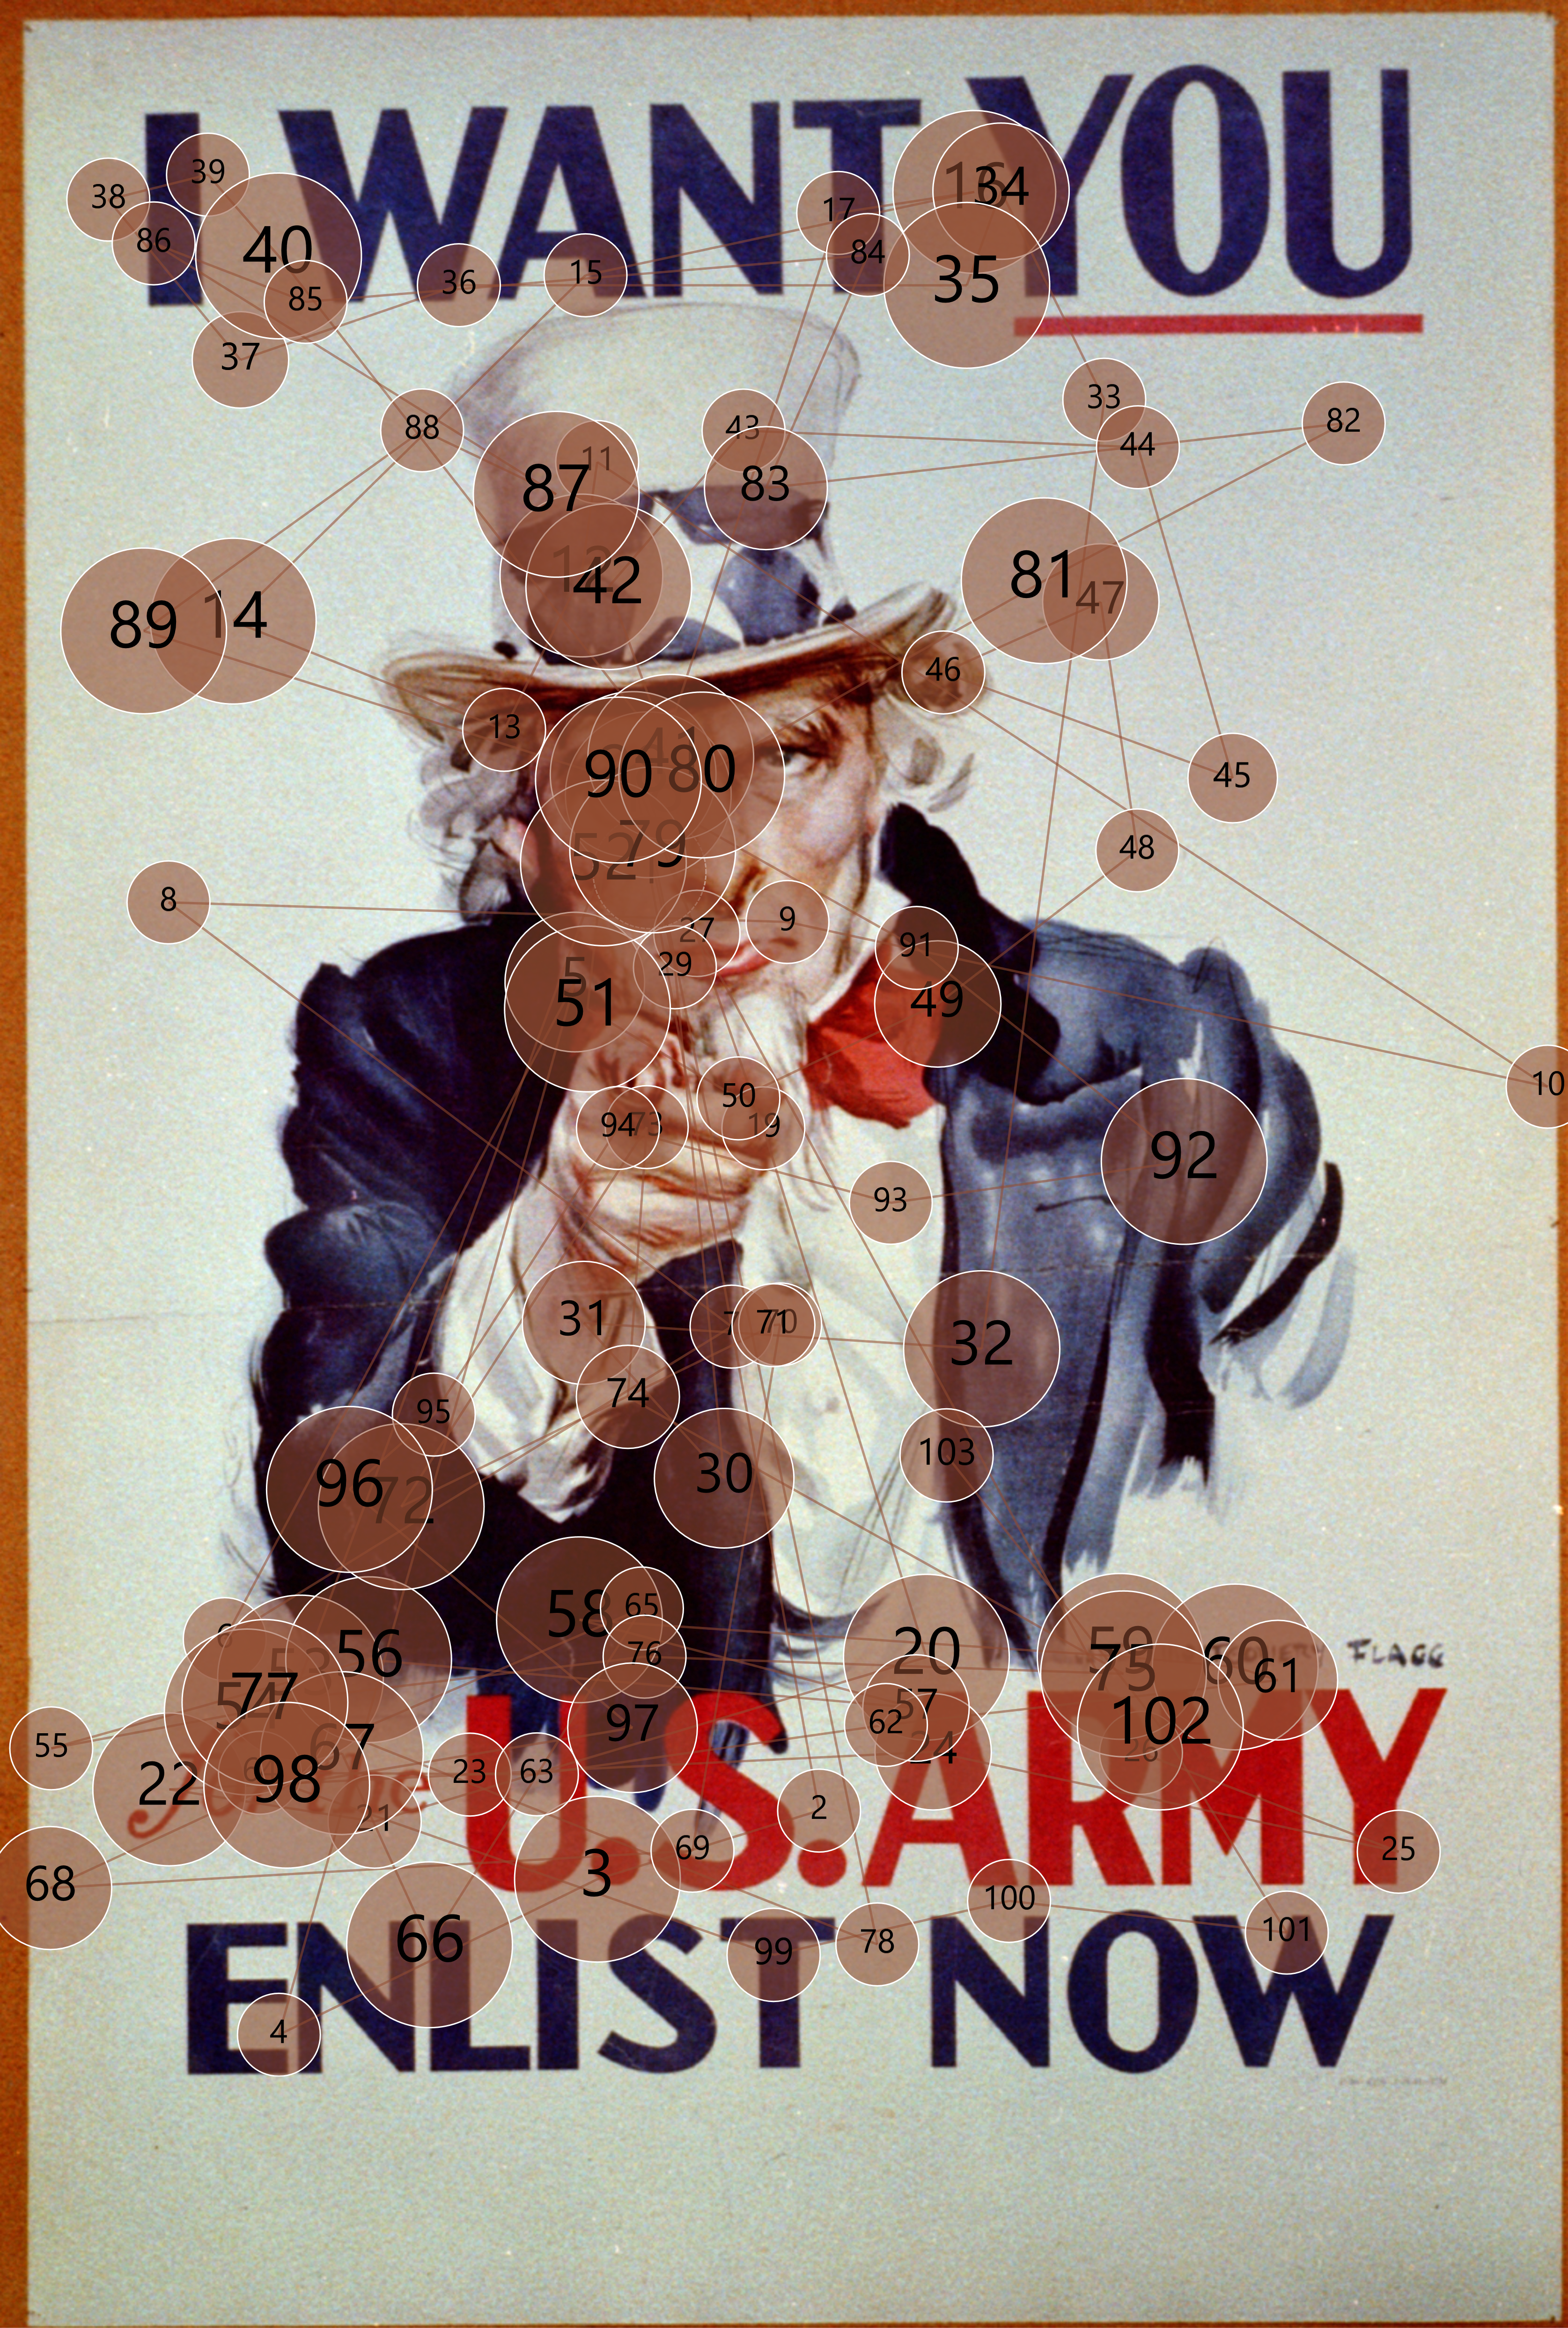
\includegraphics[keepaspectratio,width=\textwidth]{../../12_DataAnalysis/GazePlot.png}
        \subcaption{Gaze Plot}
    \end{minipage}
    \begin{minipage}[b]{.48\textwidth}
        \centering
        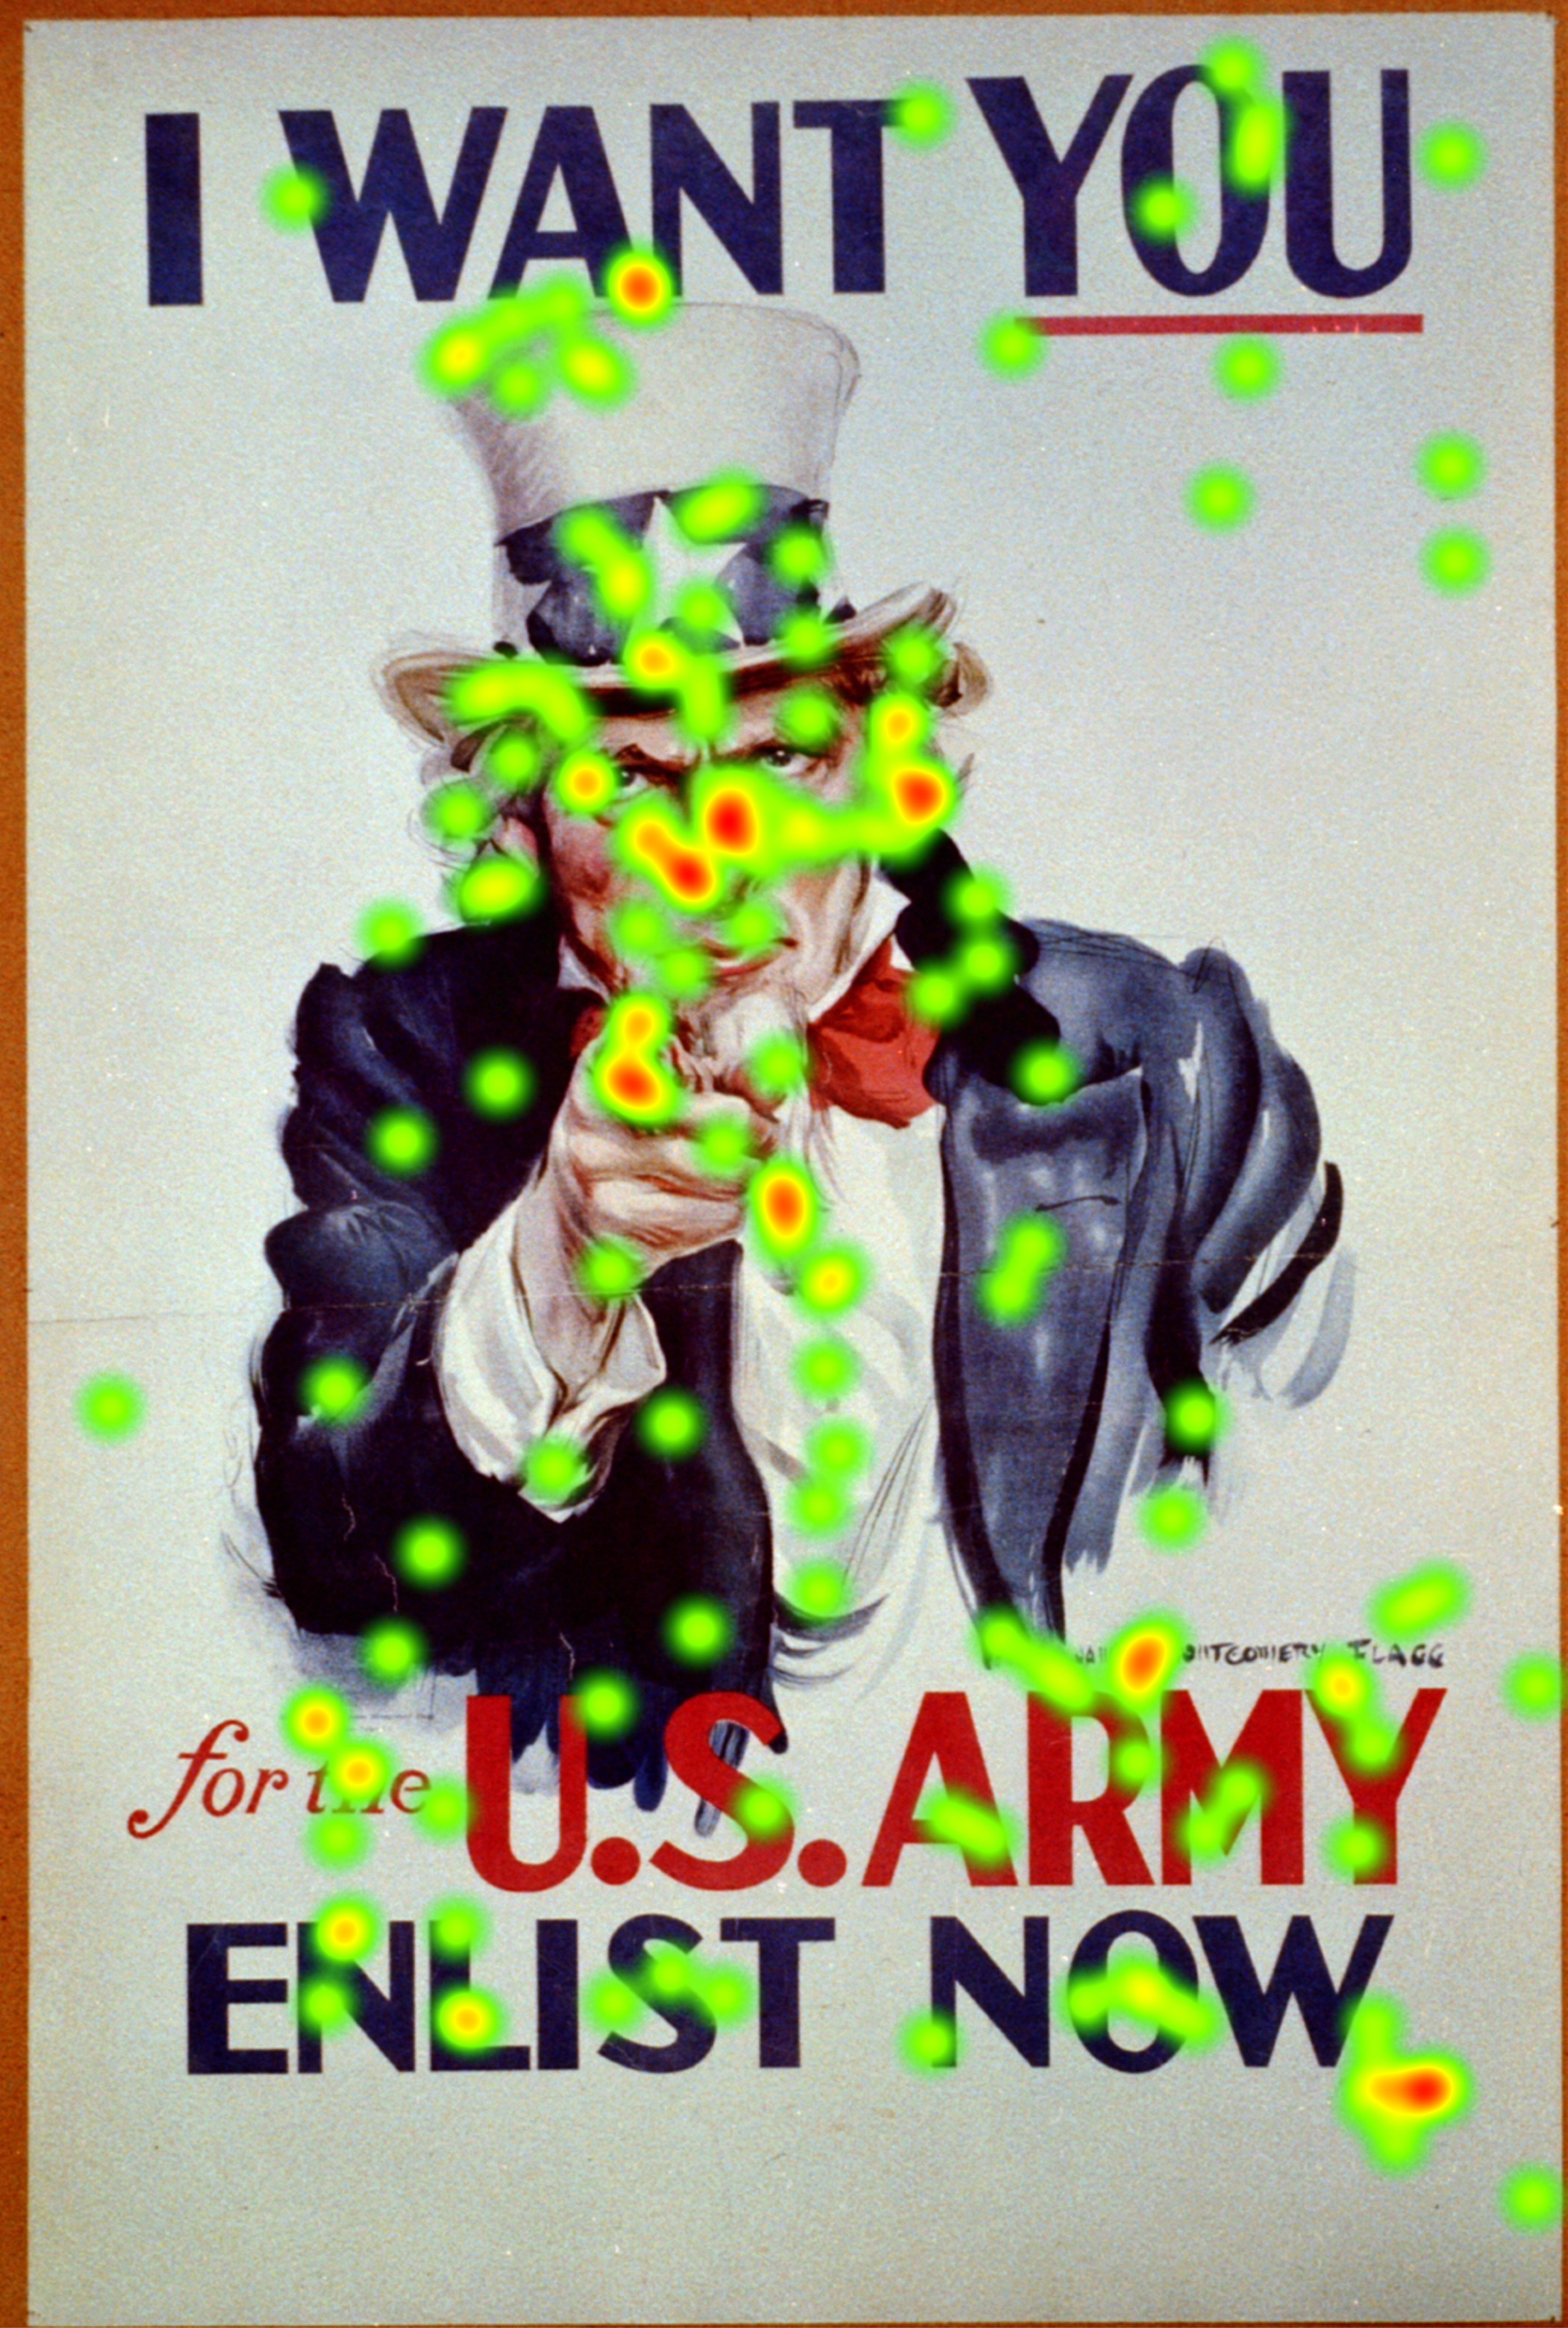
\includegraphics[keepaspectratio,width=\textwidth]{../../12_DataAnalysis/HeatMap.png}
        \subcaption{Heat Map}
    \end{minipage}
    \caption{\kadaid \ 実験結果}
    \label{fig:実験結果\kadaid}
\end{figure}
\section{\consideration}
我々はポスターを見るときに,文字情報や被写体が印象に残る.
結果より,文字や被写体の顔部分をより多く注視しているからではないだろうか.
注視した順番については,全体的に偏りは見られないものの,文字列に対しては比較的小さい数値が出力されている.
我々は,まず文字から情報を得ようとするのではないだろうか.
\section{\conclusion}
本実験を通して,刺激画像の注視箇所と我々の印象に残っている点の因果を考察できた.
しかし,差された指の指先も注目すべき注視箇所だが,なぜ指先が多く注視されているのかの原因は分からなかった.
\bibliography{bib}
\chapter*{付録}
\addcontentsline{toc}{chapter}{付録}
\setcounter{section}{0}
\renewcommand{\thelstlisting}{src.\thesection-\arabic{lstlisting}}
\renewcommand{\thesection}{\Alph{section}}
\section{課題1}
\lstinputlisting[caption={01-01: \kadaiaa},label={src:01_01}]{../../01_EngineeringCharacteristicsOfSound/no1.m}
\lstinputlisting[caption={01-02: \kadaiab},label={src:01_02}]{../../01_EngineeringCharacteristicsOfSound/no2.m}
\end{document}